\documentclass{Preparation}
\def\titre{Préparation à l'examen 3}
\def\soustitre{À l'intention des étudiants du cours MAT-2901 : Mathématiques et technologie}
\def\auteur{J\'er\^ome Soucy}

\def\DateHeure{}
\def\Ponderation{}

\usepackage{commandesJS}
\usepackage{array}					% Pour mon tableau de la question 6.
\usepackage{multirow}				% Pour mon tableau de la question 6.
\usepackage{graphicx}
\usepackage{siunitx}
\sisetup{
	output-decimal-marker={,},
	group-separator={\,},
}
\usepackage{pgf,tikz}	% Utilisation du module tikz, qui permet de tracer des belles images
	\usetikzlibrary{automata, positioning} % Pour tracer le graphe de la question 2
\begin{document}
\pagecouverture
\section{Détails de l'évaluation}
\begin{itemize}
	\item Date et heure : Sur le site du cours, rendez-vous dans la section \textit{Évaluations et résultats}~$\rightarrow$~\textit{Examen 3}
	\item Pondération : Sur le site du cours, rendez-vous dans la section \textit{Évaluations et résultats}~$\rightarrow$~\textit{Examen 3}
	\item Local : Sur le site du cours, rendez-vous dans la section \textit{Évaluations et résultats}~$\rightarrow$~\textit{Examen 3}
	\item Matière à l'étude
		\begin{itemize}
			\item Série 10 : Processus stochastiques (1/3)
			\item Série 11 : Processus stochastiques (2/3)
			\item Série 12 : Processus stochastiques (3/3)
			\item Série 13 : Localisation
			\item Série 14 : Couteau gamma
		\end{itemize}
    \item Matériel requis
		\begin{itemize}
			\item Crayon et efface
			\item Règle graduée en centimètres
            \item Calculatrice autorisée par la \textsc{fsg} (voir le site de cours pour connaître les modèles autorisés)
		\end{itemize}
	\item Aucun matériel ne sera fourni avec l'évaluation
\end{itemize}
\newpage
\section{Questions préparatoires}
\begin{question}
Yohan a une façon très markovienne de choisir ses dîners. Il ne mange que l’un des cinq plats suivants : macaroni (M), pizza (P), pâté chinois (C), poulet général Tao (T) ou sushis (S). Si Yohan \textbf{n’a pas mangé de sushis la veille}, il lance un dé à 6 faces pour déterminer son repas. Si le résultat est un 6, il mange des sushis. Dans ce cas, il ignore complètement ce qu’il a mangé la veille. En revanche, \textbf{s’il a mangé des sushis la veille}, il ne veut surtout pas en remanger deux jours de suite — question de budget ! Il lance alors un dé à 4 faces, identifiées par M, P, C et T. Le résultat indique directement son repas du jour. Dans tous les autres cas (c’est-à-dire s’il \textbf{n’a pas mangé de sushis la veille et qu’il n’obtient pas un 6 au dé}), le repas de Yohan est déterminé en fonction du repas de la veille, selon le graphe de transition ci-dessous. Par exemple, s’il a mangé du macaroni hier et qu’il ne tombe pas sur un 6, il mangera aujourd’hui :
\begin{itemize}
    \item du poulet général Tao avec une probabilité de $1/3$,
    \item du pâté chinois avec une probabilité de $1/3$,
    \item ou de la pizza avec une probabilité de $1/3$.
\end{itemize}

S’il avait plutôt mangé du pâté chinois et qu’il ne tombe pas sur un 6, alors il mangera inévitablement de la pizza, et ainsi de suite selon le graphe.
\begin{center}
	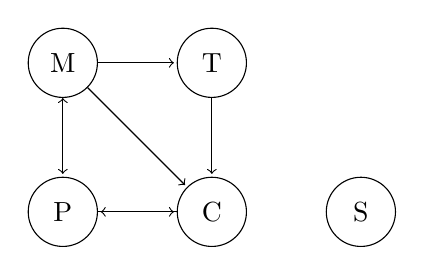
\begin{tikzpicture}
	\node[state]             (1) {M};
	\node[state, below=of 1] (2) {P};
	\node[state, right=of 2] (3) {C};
	\node[state, right=of 3] (4) {S};
	\node[state, right=of 1] (6) {T};
	
	\draw[every loop]
	(1) edge[<->]   (2)
	(1) edge[]   (6)
	(1) edge[]  (3)
	(3) edge[]  (2)
	(2) edge[]  (3)
	(6) edge[]  (3);
	\end{tikzpicture}
\end{center}

\begin{parts}
	\part Trouvez la matrice décrivant les probabilités de transition entre les différents repas.
	\part Soit $P$ la matrice trouvée en (a). Utilisez un outil informatique pour trouver un vecteur $\vec{v}$ tel que $A\vec{v}=\vec{v}$.
	\part Déterminez la fréquence à long terme de chacun des repas dans les choix de dîner de Yohan.
\end{parts}

\end{question}
\begin{question}
Gilberte et Marcelle sont deux jeunes femmes botswanaises inscrites sur le site de rencontres \textit{Trouve ton lorato}\footnote{\textit{Lorato} signifie « amour » en tswana, la langue majoritairement parlée au Botswana.}. Toutes deux discutent avec un certain Kevin, et elles aimeraient savoir dans quel coin du Botswana il habite. D’après le site, Gilberte se trouve à 4 km de Kevin, tandis que Marcelle est à 5 km de lui.

Marcelle habite à l’origine d’un repère cartésien, et Gilberte réside au point $(-1, 4)$. Les coordonnées sont exprimées en kilomètres.

\begin{parts}
\part Déterminez l’ensemble des points où Kevin pourrait habiter, en supposant que les distances données par le site sont exactes.

\part Pour localiser précisément Kevin, Gilberte et Marcelle demandent à leur amie Brenda de s’inscrire elle aussi sur le site, afin de connaître la distance qui la sépare de Kevin. Sachant que Gilberte et Marcelle connaissent déjà la position de Brenda, pourront-elles déterminer avec certitude l’emplacement exact de Kevin? Justifiez votre réponse, en supposant toujours que les distances données sont exactes.

\part Que se passe-t-il si Brenda est la voisine d’appartement de Marcelle, et que la précision du site sur les distances est d’environ 1 km? Expliquez brièvement.
\end{parts}
\end{question}
    
  \begin{question}
  Considérons la matrice suivante:
  \[
P = 
\begin{pmatrix}
1   & 0   & 0   & 0 & 0 \\
0   & 1   & 0   & 0 & 0 \\
0   & 0   & \sfrac{1}{2} & 0 & 0 \\
0   & 0   & \sfrac{1}{2} & 1 & 0 \\
0   & 0   & 0   & 0 & 1
\end{pmatrix}.
\]
\begin{parts}
\part Trouvez les valeurs propres de $P$.
\part Trouvez les vecteurs propres associés à la valeur propre 1 de $P$.
\part Dessinez un mini-web qui possède $P$ comme matrice de transition.
\part Modifiez $P$ pour que l'algorithme PageRank permette la téléportation avec probabilité $\num{0,1}$.
\end{parts}
  \end{question}
    
  \begin{question}
   Trouvez le squelette de la région située au-dessus de la courbe $y=1+\frac{1}{2}x^2$, qui est représentée ci-dessous.\
	\begin{center}
		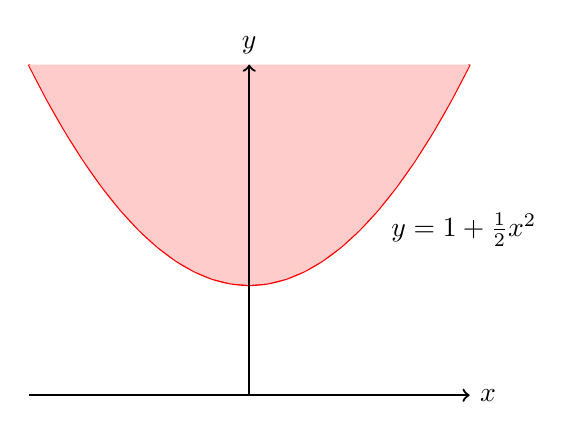
\begin{tikzpicture}[scale=1.4]
		%		\draw[step=0.5,black!20,thin] (-1.49,-1.2) grid (1.49,1.39);
		
		\draw[scale=1,domain=-2:2,smooth,variable=\x,red,thick]  plot ({\x},{1+0.5*\x*\x});
		\fill[fill=red!20] (-2,3) -- plot [domain=-2:2] (\x,{1+0.5*\x*\x}) -- (2,3) -- cycle;
		\draw[->,thick,color=black] (-2,0.) -- (2,0.) node[right] {$x$};
		\draw[->,thick,color=black] (0.,0) -- (0.,3) node[above] {$y$};
		\node[right] (A) at (1.2,1.5){$y=1+\frac{1}{2}x^2$};
		\end{tikzpicture}\\
	\end{center}
   \end{question}
\end{document}
